\chapter{Vorstellung Streaming Frameworks}
\label{chapter:vorstellung}

In Kapitel \ref{chapter:grundlagen} und \ref{chapter:analyse} wurden Grundlagen geschaffen, eine Analyse durchgeführt und ein Referenzmodell mit Bewertungskriterien vorgestellt und für die Anwendung auf die Streaming frameworks erläutert. In den folgenden Unterkapitel werden die einzelnen Streaming frameworks Apache Storm, Apache Kafka, Apache Flume und Apache S4 vorgestellt. Jedes Unterkapitel beginnt zuerst mit einer Übersicht über das Streaming framework. Anschließend wird kurz auf die Entstehung des Streaming frameworks bis zum Zeitpunkt der Erstellung dieser Thesis eingegangen. Nach der kurzen Übersicht werden die Bewertungskriterien aus Liste \ref{liste:bewkrit} auf das Streaming framework angewendet. Dabei wird wie in der Analyse des Referenzmodells vorgegangen. Eine kurzer Vergleich zwischen dem Referenzmodell wird am Ende des Unterkapitels eines Streaming frameworks durchgeführt.

\section{Apache Storm}
\label{section:storm}

Apache Storm wird vom Hauptentwickler Nathan Marz im Proposal als verteiltes, fehlertolerantes und hochperformantes Echtzeitberechnungssystem definiert. Ursprünglich wurde die Anwendung von der Firma Backtype in 2011 entwickelt. Im gleichen Jahr wurde die Firma Backtype von Twitter übernommen und der Quelltext auf Github \citeint{GitHub} unter dem Repository \textit{storm} \citeint{storm:GitHub} von Nathan Marz veröffentlicht. In 2013 wurde die Aufnahme von Storm in die \gls{glo:asf} geplant. Dazu wurde ein Storm Proposal von Nathan Marz eingereicht. \citeint{storm:apache:stormProposal} 

Seit 2013 befindet sich Storm im Apache Incubation-Prozess \citeint{storm:apache:stormIncubationStatus}. Eine Überführungsversion 0.9.1-incubating wurde dafür eingerichtet. Der Quelltext und das Lizenzmodell wird in die \gls{glo:asf} aufgenommen \citeint{apache:softwareFoundation}. Der Verlauf des Überführungsprozesses zur \gls{glo:asf} wird auf der Incubator-Statusseite \citeint{storm:IncubatorStatusPage} festgehalten. In der Tabelle \ref{tab:vorstorm} wird eine Kurzübersicht über Apache Storm gegeben. Darin wird ein aktiver Entwicklungsstatus angegeben. Die Aktivität wird aus dem GitHub \textit{Contributors-Graph} bei 84 Projektteilnehmern bestimmt \citeint{storm:Contributors}. Zur Entwicklung werden mehrere Sprachen Clojure, Java und Python angegeben. Nathan Marz gibt an Storm in der Programmiersprache Clojure \citeint{clojure} zu entwickeln und mit Java  \citeint{javaAbout} kompatibel zu sein, neben Java und Clojure  findet die Github Sprachen-Suche \citeint{storm:GitHubApacheMirror} im Repository \textit{storm} auch Python \citeint{pythonAbout}. Ab Version 0.9.1-incubating wird eine verbesserte Plattformkompatibilität zum Betriebssystem Microsoft Windows angeboten und die Standardtransportschicht ZeroMq \citeint{zeromq:guide} wurde durch Netty \citeint{netty} ersetzt \citeint{storm:Changelog}.

\begin{table}[htbp]
	\centering
		\begin{tabular}{@{}ll@{}} \toprule
			\textbf{Faktum} & \textbf{Beschreibung} \\ \midrule
			Hauptentwickler & Nathan Marz \\
			Stabile Version & 0.9.1-incubating vom 22.02.2014 \\ 
			Entwicklungsstatus &  Aktiv \\
			Entwicklungsversion & 0.9.2-incubating, 0.9.3-incubating \\
			Sprache & Clojure, Java, Python \\
			Betriebssystem & Platformübergreifend (Microsoft Windows mit Cygwin Umgebung) \\
			Lizenz & Eclipse Public License 1.0 (Incubating Apache License version 2.0) \\
			Webseite &  \citeint{storm:home} \\
			Quelltext & \citeint{storm:GitHubApacheMirror} \\			
			\bottomrule			
		\end{tabular}
	\caption{Kurzübersicht Apache Storm}
	\label{tab:vorstorm}
\end{table}

In Tabelle \ref{tab:bewstorm} werden die Bewertungskriterien aus Kapitel \ref{chapter:kriterien} in Apache Storm geprüft. Als Architektur wird die moderne Systemarchitektur Strukturierte Peer-To-Peer-Architektur, die eine horizontale Verteilung unterstützt, angegeben. Apache Storm besteht aus drei Komponenten: \textit{Nimbus}, \textit{Supervisor} und \textit{UI}. Der \textit{Nimbus} stellt die zentrale Stelle und übernimmt die Aufgabe des \textit{Scheduler} - einem Arbeitsplaner. Der \textit{Nimbus} is klein gehalten und verteilt die Aufgaben zwischen den Arbeitsknoten. Die Arbeitsknoten werden in Apache Storm \textit{Supervisor} genannt. Mehrere Supervisor-Instanzen sind in einem Apache Storm Cluster möglich. Die dritte Komponente \textit{UI} visualisiert den momentanen Status der Apache Storm Komponenten \textit{Nimbus} und \textit{Supervisor}. 

Bei der Verarbeitung von Informationen kann in Apache Storm pro Verarbeitungseinheit die Anzahl an benötigten Threads als Argument explizit übergeben werden. Die Konfiguration dazu findet im Quelltext statt. Um eine komplexe Verarbeitung durchzuführen, muss in Apache Storm eine \textit{Topology} implementiert und veröffentlicht werden. Die \textit{Topology} wird auf dem Apache Storm Cluster permanent ausgeführt und kann nicht dynamisch verändert werden. Die Kommunikation erfolgt zwischen den einzelnen Apache Storm Komponenten mit einem zusätzlichen Werkzeug: Apache ZooKeeper \citeint{zookeeper:Home}. Apache ZooKeeper wird als verteilte Synchronisation und Koordination der Aufgaben durch Nimbus auf tieferer Ebene verwendet. Auf der Transportebene kommunizieren Verarbeitungseinheiten durch das asynchrone Client-Server-Framework Netty \citeint{netty}.

Eine komplexe Verarbeitung bzw. Abfrage in einer \textit{Topology} besteht aus \textit{Spouts} und \textit{Bolts}. Die Kommunikation ist dabei einseitig. Ein Empfänger-\textit{Bolt} kann keine Nachricht an einen Sender-\textit{Bolt} zurück schicken. Mit einem \textit{Spout} wird eine externe Datenquelle beschrieben und ein \textit{Spout} liefert eine permanente Folge von ungebunden Tupeln. Ein Tupel ist die Hauptdatenstruktur und kann unterschiedliche Datentypen (integers, longs, shorts, bytes, strings, doubles, floats, booleans und selbstentwickelte) enthalten. Die Folge von ungebundenen Tupeln wird in Apache Storm als \textit{Stream} bezeichnet. Um einen \textit{Spout} zu implementieren reicht es die Schnittstelle \textit{IRichSpout} zu implementieren oder die Klasse \textit{BaseRichSpout} zu erweitern. 

Bei einer Erweiterung von \textit{BaseRichSpout} sind mindestens die Methodenamen \textit{open}, \textit{nextTuple} und \textit{declareOutputFields} zu implementieren. In der Methode \textit{open} kann zum Beispiel eine interne Liste über einen Java-Listener bei einem Dateneingang in einem Datenadapter gefüllt werden. Die Methode \textit{nextTuple} wird jede erste Millisekunde ausgeführt und wenn Nachrichten in der Liste enthalten sind, kann der \textit{SpoutOutputCollector} einen Stream mit einer eindeutigen StreamId und einem Tuple aussenden. Wenn die Nachricht nicht vollständig übertragen wurde, wird über ein \textit{Callback-Methode} \textit{ack} oder \textit{fail} in der implementierten Klasse \textit{Spout} zurückgegeben. Damit wird in Apache Storm sichergestellt, dass die Nachricht mindestens einmal vollständig verarbeitet wurde \citeint{storm:SpoutOutputCollector}. In der Methode \textit{declareOutputFields} wird die Felddefinition der Ausgabe für die weitere Verarbeitung angegeben. \citeint{storm:Spout}

Ein \textit{Bolt} nimmt ein Tupel auf und gibt Tupel wieder aus. Innerhalb eines \textit{Bolt} können Tupel verändert werden. Nachdem Start der \textit{Topology} wird ein \textit{Bolt} erst auf den \textit{Supervisor} übertragen und deserialisiert. \textit{Nimbus} ruft auf der Instanz anschließend die Methode \textit{prepare} auf. In Java muss für die Implementierung eines \textit{Bolt} die Schnittstelle \textit{IBolt} oder \textit{IRichBolt} implementiert werden. Alternativ können auch Basisimplementierungen verwendet werden, wie zum Beispiel \textit{BaseBasicBolt} oder \textit{BaseRichBolt}. Mit der Methode \textit{execute} werden die Tupel angepasst und über den \textit{OutputCollector} ausgesendet. Apache Storm erwartet beim Eingang eines Tupels in einem \textit{Bolt} Bestätigung über die Methode \textit{ack} oder \textit{fail}. Andernfalls kann Apache Storm nicht feststellen, ob eine Nachricht vollständig verarbeitet wurde. \citeint{storm:Bolt}

\begin{figure}[htb!]
\centering
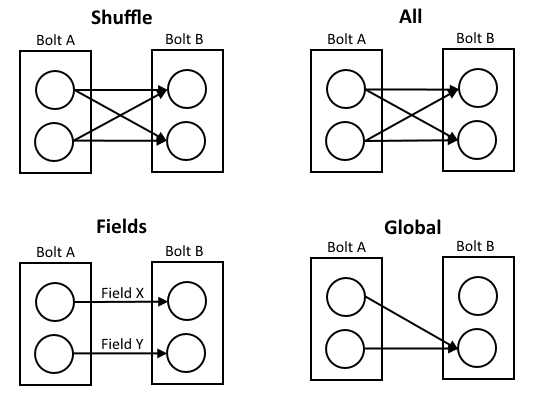
\includegraphics[width=1.0\textwidth]{bilder/stormGroupings.png}
\caption{Apache Storm Gruppierungen
\label{fig:stormGroupings}}
\end{figure}

Durch den \textit{TopologyBuilder} kann eine komplexe Abfrage aus \textit{Spouts} und \textit{Bolts} zusammengesetzt werden. Der \textit{TopologyBuilder} stellt dazu \textit{set}-Methoden für \textit{Spouts} und \textit{Bolts} bereit. Bei dem Setzen eines \textit{Spout} oder eines \textit{Bolt} muss immer eine Referenz-Identifikationsnummer angegeben werden. Durch die Referenz können \textit{Bolt}- oder \textit{Spout}-Komponenten untereinander verbunden werden. Weiterhin kann mit dem Argument \textit{parallelism\_hint} die Anzahl der \textit{Tasks} eingestellt werden, die zur Ausführung benutzt werden. Jeder \textit{Task} wird im Storm Cluster auf einem eigenen \textit{Thread} ausgeführt. Wenn die \textit{setBolt}-Methode aufgerufen wird, wird ein Objekt \textit{InputDeclarer} erzeugt. Darin können verschiedene Gruppierungen (\textit{Shuffle}, \textit{Fields}, \textit{All}, \textit{Global}, \textit{None}, \textit{Direct}, \textit{LocalOrShuffle} \citeint{storm:InputDeclarer}) angegeben werden, um den Stream in definierte Teile zu trennen. In Abbilung \ref{fig:stormGroupings} werden Vier Standardgruppierungen in Apache Storm gezeigt. Mit einem \textit{ShuffleGrouping} werden Tupel eines \textit{Stream} zufällig über die \textit{Tasks} verteilt. Beim \textit{FieldsGrouping} wird der \textit{Stream} durch die Angabe eine Schlagworts getrennt. Tupel mit dem gleichen Schlagwort werden immer an den gleichen \textit{Task} gesendet. Das \textit{AllGrouping} wird auf allen Tasks des \textit{Bolt} repliziert und beim \textit{GlobalGrouping} wird der \textit{Stream} zu einem \textit{Task} gesendet. Weiterhin gibt es noch das \textit{NoneGrouping} bei dem der \textit{Stream} auf dem gleichen \textit{Task} ausgeführt wird und beim \textit{DirectGrouping} entscheidet der \textit{Stream}-Erzeuger auf welchen Konsumenten-\textit{Task} der \textit{Stream} gesendet wird. Durch die Schnittstelle \textit{CustomStreamGrouping} is eine weitere konkrete Implementierung für eine \textit{Grouping}-Strategie möglich. \citeint{storm:TopologyBuilder}

In Apache Storm wird eine Abstraktion \textit{Trident} für eine transaktionsorientierte Abfrage- und Datenverarbeitung bereitgestellt. Mit \textit{Trident} ist es möglich eine Stapelverarbeitung mit Statusinformationen durchzuführen. Es gibt Fünf Ausführungstypen: \textit{Partition-local}, \textit{Repartitioning}, \textit{Aggregation}, \textit{GroupedStreams} und \textit{Merges and Joins}. In \citeint{storm:Trident} wird \textit{Trident} näher erläutert. In den folgenden Absätzen wird kurz auf die möglichen Funktionen mit \textit{Trident} aus \citeint{storm:Trident} eingegangen.

Unter \textit{Partition-local} werden Operatoren (\textit{function}, \textit{filter}, \textit{partitionAggregate}, \textit{partitionPersist}, \textit{projection}) lokal in einem Stapelelement ausgeführt. Die Operatoren \textit{function} und \textit{filter} erben jeweils von der gleichen Basisklasse \textit{BaseFunction}. Bei den Methoden \textit{partitionAggregate} und \textit{partitionPersists} können unterschiedliche Strategien entwickelt werden. Ein neues Aggregat kann mit der \textit{Aggregator}-Schnittstelle oder den erweiterten Schnittstellen \textit{CombinerAggregator} oder \textit{ReducerAggregator} implementiert werden. Um nicht im bestehenden Arbeitsspeicher mit der \textit{MemoryMapState.Factory()} Daten zu speichern, kann über eine konkrete Implementierung der Schnittstelle \textit{IBackingMap} eine neue Strategie zur Datenablage erzeugt werden. Mit \textit{Projection} können Teile der Felder aus einem \textit{Stream} in einem neuen \textit{Stream} unverändert abgebildet werden.

Beim \textit{Repartitioning} kann die Stapelverarbeitung durch \textit{Repartitioning}-Funktionen (\textit{shuffle}, \textit{broadcast}, \textit{partitionBy}, \textit{global}, \textit{batchGlobal}, \textit{partition}) geändert bzw. neu strukturiert werden. Zum Beispiel kann sich die Anzahl der \textit{Tasks} zur parallelen Datenverarbeitung ändern. Mit dem \textit{Repartitioning} ist es möglich die \textit{Tasks} im Cluster neu zu verteilen. Die Methode \textit{groupBy} nutzt \textit{Repartitioning} um den \textit{Stream} mit \textit{partitionBy} neu zu strukturieren. Gruppierte und aggregierte \textit{Streams} können mit bestehenden Apache Storm Primitiven verkettet werden.

\textit{Streams} können in \textit{Trident} durch die spezielle \textit{TridentTopology} zusammengeführt werden. Die \textit{TridentTopology} bietet dazu die Methoden \textit{merge} und \textit{join} an. Beide Methoden erzeugen jeweils einen neu kombinierten \textit{Stream}. Eine Zusammenführung in einem Zeitfenster, dem \textit{Windows Join}, kann mit Hilfe von \textit{partitionPersist} und \textit{stateQuery} durchgeführt werden. Mit \textit{partitionPersist} wird ein \textit{Stream} nach der Identität, die im \textit{join} referenziert wird, zerlegt und in einem Statusstapel mit der Methode \textit{makeState} in der \textit{TridentTopology} ein Status erzeugt werden. Der neue \textit{Stream} steht dadurch permanent für eine Stapelverarbeitung über das \textit{stateQuery} durch \textit{lookup}-Abfragen auf die Identität bereit. 

In der Archivdatei des Quelltextes von Apache Storm \citeint{storm:GitHubApacheMirror} ist im Unterverzeichnis \textit{Example} eine Beispielanwendung \textit{\textit{WordCountTopology.java}} vollständig hinterlegt. Im Anhang \ref{section:quelltext} wird dazu ein Beispiel-Quelltext \ref{lst:WordCountTopology} zum Wortzählen ausgegeben. Der Quelltext stellt einen Auszug des Java-Projekts \textit{storm-starter} aus dem gleichen Verzeichnis dar. In der Methode \textit{main} wird die \textit{Topology} mit einem \textit{RandomSentenceSpout} und Zwei \textit{Bolts}, einem \textit{SplitSentence} und einem \textit{WordCount} erzeugt. Der \textit{RandomSentenceSpout} bekommt Fünf \textit{Tasks} zugeordnet und erhält die Identität "`spout"'. Der \textit{Bolt} \textit{SplitSentence} ist eine \textit{ShellBolt} in dem das Teilen der Satzes in einzelne Worte in der externen Programmiersprache Python über die Kommandozeile angestoßen wird. Beim ersten \textit{Bolt} wird \textit{SplitSentence} auf den \textit{Stream} "`spout"' mit Acht \textit{Tasks}, einem \textit{ShuffleGrouping} und der Identität "`split"' angewendet. Der zweite \textit{Bolt} nimmt den \textit{Stream} "`spout"' aus dem ersten \textit{Bolt} auf und zählt die Worte im \textit{Bolt} \textit{WordCount}, mit Zwölf \textit{Tasks}, einem \textit{FieldGrouping} und der Identität "`count"'. Das \textit{FieldGrouping} von \textit{WordCount} wird nach dem Feld "`word"' gruppiert und der Ausgabestrom enthält nach einer Verarbeitung die Anzahl eines Wortes als Schlüssel-Wert-Paar. Abschließend prüft eine Bedingung, ob die \textit{Topology} im \textit{local cluster mode} zum Debuggen, dem Fehlerlösen durch Haltepunkte, auf dem lokalen Rechner oder in einem Storm Cluster ausgeführt werden soll.

Eine \textit{Topology} hat spezielle \textit{acker}-\textit{Tasks} die die Verarbeitung der \textit{Bolts} und \textit{Spouts} überwachen. Wenn ein Abfragegraph vollständig abgearbeitet wurde, dann wird an das auslösende \textit{Spout} vom \textit{acker}-\textit{Task} die Nachricht gesendet. In dem \textit{Spout} wird die \textit{Callback}-Methode \textit{ack} oder \textit{fail} anschließend verarbeitet. Zusätzlich wird in der \textit{Storm UI} die Anzahl der Nachrichten zu \textit{ack} und \textit{fail} in der Summe dargestellt. Bei Ausfall eines Tasks bekommt der Wurzelknoten eines Abfragegraphens einen "`timeout"' und der Abfragegraph wird "`replayed"', also erneut abgearbeitet. Bei Absturz eines Spout Tasks muss das Warteschlangensystem dafür sorgen, sobald der Spout Task wieder verfügbar ist, die Nachrichten in der Quelle bereitzustellen. \citeint{storm:FullyProcessed}

\begin{table}[ht!]
	\centering
		\begin{tabular}{@{}ll@{}} \toprule
			\textbf{Kriterium} & \textbf{Bewertung} \\ \midrule
			Architektur & Strukturierte Peer-to-Peer-Architektur \\
			Prozesse und Threads & Client-Server Cluster \\
			Kommunikation & TCP-basiert mit Apache Zookeeper \\
			Namenssystem & Hierarchische Benennung \\
			Synchronisierung & Zentralisierter Algorithmus \\
			Pipelining und Materialisierung & Methodenverkettung \\
			Konsistenz und Replikation & Reliability Algorithmus \\
			Fehlertoleranz & Fail-Fast Strategie unter Supervision \\
			Sicherheit & Nur eigene Maßnahmen \\
			Erweiterung & Eigenentwicklung und Community-Beiträge \\
			Qualität & Guaranteeing message processing \\
			\bottomrule			
		\end{tabular}
	\caption{Bewertung Apache Storm}
	\label{tab:bewstorm}
\end{table}

In Apache Storm können der \textit{Worker}, die \textit{Node}, der \textit{Nimbus}- oder \textit{Supervisor}-Dienst abstürzen. Der \textit{Worker} wird vom \textit{Supervisor} neugestartet falls der \textit{Worker} einen Fehler hat. Der \textit{Nimbus} leitet die Abfrage an eine andere Maschine, wenn der \textit{Supervisor} den \textit{Worker} nicht neugestartet bekommt. Sobald eine Node ausfällt, startet \textit{Nimbus} die \textit{Tasks} auf einer anderen Maschine. Da beide Dienste in einem Fehlerfall schnell ausfallen und keinen Statusmonitor für einen Ausfall anbieten, ist ein externes \textit{Monitoring} (nagios \citeint{nagios:Monitoring}) und ein \textit{Superversion} (supervisord \citeint{supervisor:ProcessControlSystem}) der Anwendungsdienste \textit{Nimbus} und \textit{Supervisor} notwendig. Nachdem der \textit{Nimbus}- oder \textit{Supervisor}-Prozess durch den Supervisiondienst neugestartet wurde, können neue \textit{Tasks} zu den laufenden \textit{Tasks} auf den \textit{Workern} hinzugefügt werden. \citeint{storm:FaultTolerance}

Die Sicherheit unter Apache Storm wird bisher nur durch Einsatz zusätzlicher Administration des Anwendungssystems erreicht. Auf der Netzwerkebene müssen \gls{glo:ip}-Verbindungen mit \gls{glo:ipsec} gesichert werden. Eine Authentifizierung zwischen den Apache Storm Komponenten und zwischen Apache Zookeeper ist nicht vorhanden. Daher können auf der Anwendungsebene spezifische Richtlinien durch \glspl{glo:acl} umgesetzt werden. \citeint{storm:Security}

Da der Quelltext der Hauptanwendung öffentlich ist, können spezifische Implementierungen in einem separaten Repository hinzugefügt werden. Apache Storm gibt eine Garantie auf Nachrichtenverarbeitung, wie in \citeint{storm:FullyProcessed} gezeigt. Ein \gls{glo:qos} kann durch die Unterstützung des \textit{Monitoring} iterativ entwickelt werden. Ein komplexes \gls{glo:qos}-System ist in Apache Storm nicht vorhanden.

Apache Storm wurde zu Beginn kurz vorgestellt und anschließend durch die Bewertungskriterien genauer erläutert. Es wurden spezifische Begriffe in Apache Storm vorgestellt und in einer Anwendung WordCount gezeigt. Das Erstellen einer Anwendung ist in wenigen Klassen erledigt. Das Debuggen lässt sich in einem lokalen Clustermodus erledigen. Das Veröffentlichen eine Anwendung ist in einem Kommandozeilenaufruf ausgeführt. Die Sicherheit und \gls{glo:qos} sind weniger bis nicht vorhanden. Trotzdem lässt sich ein Cluster mit wenig Konfigurationsaufwand aufbauen und vertikal durch Apache Zookeeper skalieren. Im folgenden Kapitel wird Apache Kafka eingeführt.

%Monitor NASDAQ stocks between $20 and $200 that have moved down more than 2% in the last 20 minutes

\section{Apache Kafka}
%http://de.slideshare.net/tim.lossen.de/eventstream-processing-with-kafka
%http://de.slideshare.net/charmalloc/developingwithapachekafka-29910685

Nach der Vorstellung von Apache Storm wird in diesem Kapitel Apache Kafka näher gebracht. Zu Beginn wird eine Kurzübersicht gegeben, um anschließend die Bewertungskriterien zu erläutern. Apache Kafka wird von Rao in \citeint{kafka:Proposal} als verteiltes publish-subscribe Nachrichtensystem für die Verarbeitung hoher Mengen an fließenden Daten. Am 04.07.2011 wurde der Apache Incubation-Prozess aufgenommen und am 23.10.2012 wurde Apache Kafka qualifiziert \citeint{kafka:IncubationStatus}. Ursprünglich wurde Apache Kafka von der Firma LinkedIn \citeint{linkedin} um auf die eingehenden unterschiedlichen hohen Datenmengen der Webseiten von LinkedIn Zugang zu bekommen und zu verarbeiten \citeint{kafka:Proposal}.

\begin{table}[htbp]
	\centering
		\begin{tabular}{@{}ll@{}} \toprule
			\textbf{Faktum} & \textbf{Beschreibung} \\ \midrule
			Hauptentwickler & Jay Kreps, Neha Narkhede, Jun Rao \\
			Stabile Version & 0.8.1.1 vom 29.04.2014 \\ 
			Entwicklungsstatus &  Aktiv \\
			Entwicklungsversion & 0.8.2, 0.9.0 \\
			Sprache & Scala, Java, Python \\
			Betriebssystem & Platformübergreifend (Microsoft Windows mit Cygwin Umgebung) \\
			Lizenz & Apache License version 2.0 \\
			Webseite & \citeint{kafka:home} \\
			Quelltext & \citeint{kafka:GitHubApacheMirror} \\			
			\bottomrule			
		\end{tabular}
	\caption{Kurzübersicht Apache Kafka}
	\label{tab:vorkafka}
\end{table}

Die Architektur von Apache Kafka besteht aus einem Kafka Server, den \textit{Producern} und den \textit{Consumern}. Der Server stellt als \textit{Broker} die Verbindungen zwischen einem \textit{Producer} und einem \textit{Consumer} her. In einem \textit{Broker} werden \textit{Topics} registriert. Ein spezifischer Nachrichtenstrom kann durch Angabe eines \textit{Topic} bereitgestellt oder abgefragt werden. Der \textit{Producer} hält eine Liste von Verbindungen zu \textit{Brokern}. Nachrichten werden von \textit{Producern} an \textit{Broker}, wie in einem \textit{Push}-System gesendet. Bei Absturz eines \textit{Brokers} wird ein bestehender \textit{Broker} zum \textit{Master} gewählt, der zuerst aus einer Anfrage auf Aktivität antwortet. Ein \textit{Consumer} zieht Nachrichten von einem \textit{Broker}, wie in einem \textit{Pull}-System. Aktives Warten auf Dateneingang in einem "`long poll"', einem permanenten Abfragen eines \textit{Brokers} durch den \textit{Consumer}, kann durch Übergabe von Parametern in der \textit{Consumer}-Abfrage blockiert werden. Der Nachrichtenstrom stellt in einem \textit{Consumer} eine \textit{Iterator}-Schnittstelle bereit. Sobald Nachrichten eintreffen, können weiterführende Operationen ausgeführt werden. Um eine Last zu verteilen, kann ein \textit{Topic} in Partitionen aufgeteilt werden. Eine Nachricht besteht aus einem Schlüssel und einem Wert. Der Nachrichtenschlüssel kann je nach Strategie z.B. per Zufall auf bestimmte Partitionen zugeordnet werden. Partitionen sind auf Host-Maschinen in  einem Kafka-Cluster verteilt. Ein \textit{Topic} sollte in einem produktiven Einsatz die gleiche Anzahl an \textit{Threads} wie Partitionen haben. Bei geringerer Anzahl von \textit{Threads} als \textit{Topics}, entstehen Wartezeiten für \textit{Topics}. \textit{Topics} können in diesem Fall die Arbeit nicht unmittelbar starten, sondern müssen auf einen \textit{Thread}, der bereit wird, warten. Mit Kommandozeilen-Werkzeugen kann ein \textit{Rebalance} der Partitionen von \textit{Topics} in einem Kafka-\textit{Cluster} angestoßen werden. \citelit[S. 2, Kap. 3]{apache:kafka:kreps2011kafka}

\begin{figure}[htb!]
\centering
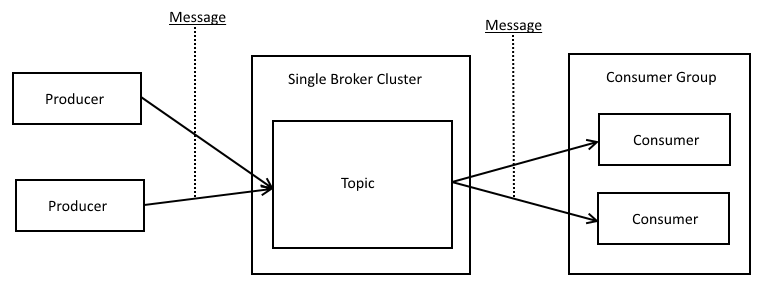
\includegraphics[width=1.0\textwidth]{bilder/kafkaDesign.png}
\caption{Apache Kafka Architektur - Single Broker Cluster
\label{fig:kafkaDesign}}
\end{figure}

Abbildung \ref{fig:kafkaDesign} zeigt ein Beispiel mit einem \textit{Single Broker Cluster} als Server. Das Kafka-Cluster kann auch aus mehreren \textit{Brokern} bestehen. Die Installationsanleitung in Anhang \ref{section:kafkainstall} zeigt eine Konfiguration für ein \textit{Single Broker Cluster}. Für ein \textit{Multi Broker Cluster} werden separate Konfigurationen der Kafka-Maschinen und ein Apache Zookeeper-Cluster benötigt. In der Abbildung \ref{fig:kafkaDesign} werden Nachrichten an das \textit{Topic} von Zwei \textit{Producern} gesendet. Aus der \textit{Consumer Group} holen Zwei \textit{Consumer} Nachrichten aus dem \textit{Topic} ab. Für die Koordination der Nachrichten greifen der \textit{Server}, die \textit{Producer} und die \textit{Consumer} im Hintergrund auf Apache Zookeeper zu. Für die horizontale Skalierung kann ein Apache Zookeeper Cluster genutzt werden. In einem Kafka-Cluster können maximal 255 Knoten existieren. Pro Konfiguration muss jeder Knoten eine eigene Identität unter der \textit{Broker-Id} festgelegt bekommen. Mehrere Knoten mit gleicher Identität führen zu einem unvorhersagbaren \textit{Cluster}-Verhalten. \citelit[S. 28]{garg2013apache}

Sobald Nachrichten von \textit{Consumern} in einem Kafka-Cluster empfangen werden, werden diese lokal innerhalb einer Apache Zookeeper-Maschine im Dateisystem gespeichert. In einem \textit{Consumer} werden die Nachrichten mit einem iterativen Zähler im \textit{Offset} gespeichert. Durch die Angabe des \textit{Offset} ist es möglich Nachrichten von einer \textit{Topic}-Partition ab einer bestimmten \textit{Offset}-Position abzuholen. Beim Speichern der Nachrichten nutzt Apache Kafka die \textit{zero-copy}-Optimierung \citelit{ibmZeroCopy}. Dabei wird die Nachricht in den Linux Page Cache einmalig geschrieben. Weitere Abfragen der Nachrichten werden vom Page Cache geliefert. Durch die zero-copy-Optimierung werden 4 context-switches pro Abfrage in einem Prozess reduziert. \citeint[Kap. 4.3]{kafka:documentation}

In Kafka wird die Reihenfolge von Nachrichten, die von einer \textit{Topic}-Partition abgeholt wird, garantiert. Die Reihenfolge von unterschiedlichen Partitionen kann allerdings abweichen und wird nicht garantiert. In Apache Kafka können Nachrichten mit der \textit{Gzip\footnote{Kompressionswerkzeug: gzip -- \url{http://www.gzip.org/}}}-Anwendung oder der \textit{Snappy\footnote{Kompressionsbibliothek: snappy -- \url{https://code.google.com/p/snappy/}}}-Bibliothek komprimiert werden. Nachrichten werden von Kafka nach einer Verarbeitung in einem \textit{Consumer} abschließend nicht gelöscht. Durch das einstellbare \gls{glo:sla} ist es möglich Nachrichten erst nach einer definierten Zeitspanne zu löschen. In einem \textit{Consumer}-Ausfall ist es durch diese Technik möglich, Nachrichten mit einem neuen bzw. bestehenden \textit{Consumer} erneut abzufragen, also Nachrichten neu einzuspielen. Dennoch sind bei der Übernahme Nachrichten-Duplikate möglich. Eine Anwendung die Kafka einsetzt und mit Duplikaten umgehen muss, muss eine Logik zur Erkennung von Duplikaten bereitstellen.
So wird beim Einsatz von mehreren \textit{Consumern} die Datenkapazität vervielfacht. Nachrichten sind verloren, falls ein \textit{Broker} mit nicht abgeholten Nachrichten ausfällt. \citelit[S. 4, Kap. 3.3]{apache:kafka:kreps2011kafka}

Aus dem Apache Kafka Archiv \citeint{kafka:GitHubApacheMirror} wurde ein Beispiel für die Verwendung von \textit{Producer} und \textit{Consumer} im Anhang unter dem Quelltext \ref{lst:kafkaProducer} und \ref{lst:kafkaConsumer} abgelegt. Beide Klassen erben von der Java \textit{Thread}-Klasse. In einer externen Klasse können beide erweiterten \textit{Threads} instanziiert und mit der \textit{start}-Methode ausgeführt werden. Im \textit{Producer}-Quelltext wird innerhalb der \textit{run}-Methode in einer Schleife eine Nachricht dauerhaft an einen übergebenen \textit{Topic} gesendet. Im \textit{Consumer}-Quelltext wird ebenfalls in der \textit{run}-Methode über ein \textit{Mapping} der \textit{KafkaStream} für das übergebene \textit{Topic} geholt und über den \textit{ConsumerIterator}, solange Nachrichten eintreffen, die Nachrichten in der Konsole ausgegeben. In beiden Implementierungen wird zuvor eine Konfiguration für das Kafka-Cluster gesetzt. Im Quelltext \ref{lst:kafkaProducer} und \ref{lst:kafkaConsumer} liegt eine hierarchische Benennung vor. Die Klasse KafkaStream liegt z.B. im Namensraum "`kafka.consumer.KafkaStream"'. Die Hierarchie wird durch den Punkt abgetrennt. Spezifiert wird von links nach rechts. Beim Synchronisieren zwischen Producer und Consumer werden über Apache Zookeeper Watcher Listener Konfigurationen aktualisiert.

\begin{table}[ht!]
	\centering
		\begin{tabular}{@{}ll@{}} \toprule
			\textbf{Kriterium} & \textbf{Bewertung} \\ \midrule
			Architektur & Strukturierte Peer-to-Peer-Architektur \\
			Prozesse und Threads & Client-Server Cluster, Consumer Pull-Modell \\
			Kommunikation & TCP-basiert mit Apache Zookeeper \\
			Namenssystem & Hierarchische Benennung \\
			Synchronisierung & Apache Zookeeper Watcher \\
			Pipelining und Materialisierung & Publishing als Consumer \\
			Konsistenz und Replikation & Replikation \\
			Fehlertoleranz & Fail-Fast Strategie unter Supervision \\ %CRC removal of bad CRCs -> self healing?
			Sicherheit & Nur eigene Maßnahmen \\
			Erweiterung & Eigenentwicklung und Community-Beiträge \\
			Qualität & At-least-once delivery, time-based \gls{glo:sla} 7 Tage \\
			\bottomrule			
		\end{tabular}
	\caption{Bewertung Apache Kafka}
	\label{tab:bewkafka}
\end{table}

Apache Kafka kann \textit{Topic}-Partitionen replizieren. Mit einem \textit{Replication}-Faktor kann die Anzahl der Replikate in der Konfiguration für einen \textit{Topic} eingestellt werden. Das erste registrierte \gls{glo:isr} bekommt die führende Rolle. Weitere Replikate übernehmen den Status des \textit{Follower}, dem Folgenden. Falls der führende \gls{glo:isr} abstürzt, wird durch den Algorithmus \textit{PacificA} \citelit{pacifica} aus den \textit{Followern} der nächste führende \gls{glo:isr} bestimmt. \citeint[Kap. 4.7]{kafka:documentation}

Da Apache Kafka auf einem Publish-Subscribe-Verfahren aufbaut ist die Wiederbenutzung bzw. Weitergabe von Nachrichten nur unter Angabe eines weiteren \textit{Topic} möglich. Dafür sind mindestens ein weiterer \textit{Publisher} und \textit{Consumer} zu implementieren. Aggregatoren und Operatoren, sowie es unter dem Referenzmodell Aurora/Borealis angeboten wird, kann unter Apache Kafka in der Hochsprache Scala oder Java in einem Producer entwickelt werden. Auch in der Sicherheit fehlen noch Anforderungen zur Authentifizierung und Verschlüsselung innerhalb des Kafka-Clusters \citeint{kafka:security}. Erweiterungen für das Monitoring werden über \gls{glo:jmx} angeboten. Eine Integration in ein Monitoringsystem wie Nagios kann mit dem Java JMX Nagios Plugin\footnote{Java JMX Nagios Plugin: check\_jmx -- \url{http://exchange.nagios.org/directory/Plugins/Java-Applications-and-Servers/check\_jmx/details}} erfolgen.

In diesem Kapitel wurde die Installation und ein Beispielanwendung für den Austausch von Nachrichten gezeigt. Auf spezielle Eigenschaften wie das zero-copy \citelit{ibmZeroCopy}, Parallelisierung und Replikation wurde eingegangen. Außerdem wurden die Bewertungskriterien aus Tabelle \ref{tab:bewkafka} für Apache Kafka erläutert. Im nächsten Kapitel wird nun Apache Flume vorgestellt.


% jkreps / benchmark-commands.txt: https://gist.github.com/jkreps/c7ddb4041ef62a900e6c

\section{Apache Flume}

Nachdem Apache Storm und Apache Kafka bewertet wurden, wird als nächstes Apache Flume vorgestellt. Apache Flume wurde ursprünglich von Jonathan Hsieh im Jahr 2009 und der Firma Cloudera entwickelt und wird als ein verteiltes, zuverlässiges und verfügbares System für effizientes Sammeln, Aggregieren und Bewegen großer Datenmengen von Protokolldaten von verschiedene Quellen zu einem Zentralen Datenspeicher beschrieben \citeint{flume:Proposal}. Am 29 Juni 2010 wurde Apache Flume unter der Apache License Version 2.0 veröffentlicht und am 20 Juni 2012 in die Apache Software Foundation überführt \citeint{flume:IncubationStatus}. Nachdem Apache Flume am 13 Juni 2013 in den Apache Incubations Prozess überführt wurde, wurde nach Version 0.9.5 in der neuen Fassung ab Version 1.0.0-incubating eine weitreichende Refaktorierung\footnote{Refaktorierung ist ein Prozess in der Software-Entwicklung, um die interne Struktur zu verbessern, während das äußere Verhalten unverändert bleibt \citelit[S. 9]{Fowler99}.} von Arvind Prabhakar, Prasad Mujumdar und Eric Sammer mit der Unterstützung von Jonathan Hsieh, Patrick Hunt und Henry Robinson durchgeführt \citeint{flume:flumeNg}. Die Abkürzung \gls{glo:ng} in der neuen Version von Apache Flume steht für die Weiterentwicklung und der Refaktorierung \citeint{flume:flumeNgRefactoring}. In dieser Arbeit wird ausschließlich die neue Fassung der Apache Foundation ab Version 1.0.0-incubating vorgestellt. In der Tabelle \ref{tab:vorflume} wird eine Kurzübersicht über Apache Flume gezeigt. Dabei wird unter den Hauptentwicklern die ersten drei Entwickler der neuen Fassung Flume-NG und abschließend die drei Entwickler aus der ursprünglichen Fassung aufgelistet.

Apache Flume wurde aus der Anforderung heraus als ein allgemeines Werkzeug Daten für einen Datenlieferanten für Apache Hadoop\footnote{Apache Hadoop ist eine Bibliothek von Anwendungen für das verteilte Rechnen von großen Datenmengen in einem Cluster. Es besteht aus dem Dateisystem \gls{glo:hdfs}, dem Algorithmus MapReduce und dem Aufgabenplaner Yarn. \citeint{hadoop:home}} entwickelt. In der Entwicklung von der Apache Flume wird gleichzeitig eine Anbindung an das Apache Hadoop Dateisystem \gls{glo:hdfs} als \textit{HDFS Sink} bereitgestellt. Dennoch sind weitere Sink-Implementierungen gegeben und möglich. In dieser Arbeit steht der Fokus in der kontinuierlichen Datenverarbeitung, weshalb die Schnittstelle zu Apache Hadoop nicht näher beleuchtet wird. \citelit[S. 1]{flumeDistributed}

\begin{table}[tbp]
	\centering
		\begin{tabular}{@{}ll@{}} \toprule
			\textbf{Faktum} & \textbf{Beschreibung} \\ \midrule
			Hauptentwickler & Arvind Prabhakar, Prasad Mujumdar, Eric Sammer \\
			& Jonathan Hsieh, Patrick Hunt, Henry Robinson \\
			Stabile Version & 1.5.0.1 vom 16.06.2014 \\ 
			Entwicklungsstatus &  Aktiv \\
			Entwicklungsversion & 1.6.0 \\
			Sprache & Java \\
			Betriebssystem & Linux/Unix konform, kein Support für Windows  \\
			Lizenz & Apache License version 2.0 \\
			Webseite & \citeint{flume:home} \\
			Quelltext & \citeint{flume:GitHubApacheMirror} \\			
			\bottomrule			
		\end{tabular}
	\caption{Kurzübersicht Apache Flume}
	\label{tab:vorflume}
\end{table}


Die Architektur von Apache Flume besteht aus mehreren einzelnen Maschinen die als \textit{Agents} bezeichnet werden. Jedem \textit{Agent} wird über eine Konfigurationsdatei die Verbindung zu einem anderen \textit{Agent} angegeben. Ein \textit{Agent} besteht immer aus einer Quelle \textit{Source}, einem Kanal \textit{Channel} und einer Ausgabe \textit{Sink}. Zwischen der \textit{Source}, dem \textit{Channel} und dem \textit{Sink} werden Nachrichten die \textit{Flume events} ausgetauscht. Daten werden von der \textit{Source} in \textit{Flume events} umgewandelt und an einen oder mehrere \textit{Channels} geschrieben. Ein \textit{Channel} ist der Bereich in dem \textit{Events} gehalten und weiter an die den \textit{Sink} gereicht werden. Der \textit{Sink} erhält ausschließlich Events von einem \textit{Channel}. In einem Agent kann es mehrere \textit{Sources}, \textit{Channels} und \textit{Sinks} geben.

\begin{table}[ht!]
	\centering
		\begin{tabular}{@{}ll@{}} \toprule
			\textbf{Kriterium} & \textbf{Bewertung} \\ \midrule
			Architektur & Strukturierte Peer-to-Peer-Architektur \\
			Prozesse und Threads & Client-Server-Modell und \gls{glo:rpc} \\
			Kommunikation & Streamorientierter synchroner Übertragungsmodus \\
			Namenssystem & Hierarchische Benennung \\
			Synchronisierung & Dezentraler Algorithmus \\
			Pipelining und Materialisierung & Agent chaining \\
			Konsistenz und Replikation & Replikation und Multiplexing \\
			Fehlertoleranz & Load balancing und Failover \\ 
			Sicherheit & FileChannel Verschlüsselung, \\
			& vereinzelte \acrshort{glo:sasl}-Sink-Integration \\
			Erweiterung & Eigenentwicklung und Community-Beiträge \\
			Qualität & FileChannel \gls{glo:wal} \\
			\bottomrule			
		\end{tabular}
	\caption{Bewertung Apache Flume}
	\label{tab:bewflume}
\end{table}

%Instead of focusing on analytics, Flume focuses primarily upon data transport and integration with a wide set of data sources and data destinations.
%http://www.ibm.com/developerworks/opensource/library/bd-flumews/index.html
%http://blog.cloudera.com/blog/2013/01/how-to-do-apache-flume-performance-tuning-part-1/
%\citelit{rfc4422}

\section{Apache S4}


Nach der Vorstellung von Apache Storm, Kafka und Flume wird in diesem Kapitel Apache S4 vorgestellt. Apache S4 ist eine Abkürzung und steht für Simple Scalable Streaming System und wird von Flavio Junqueira als allgemeine, verteilte, skalierbare, teilweise fehlertolerante und steckbare Plattform bezeichnet \citeint{s4:Proposal}. Zunächst soll eine Kurzübersicht einen ersten Einblick in Apache S4 geben. Anschließend werden die Bewertungskriterien erläutert und vorgestellt.

Die Architektur von Apache S4 baut auf einem Apache Zookeeper Cluster auf und besteht aus mehreren Apache S4 \textit{Cluster}, \textit{Processing Nodes}, \textit{Apps}, \textit{Processing Elements} und dem \textit{Communication Layer}. \textit{Apps} sind Java Archive, die in einem Apache S4 \textit{Cluster} bereitgestellt werden. Die Größe eines \textit{Clusters} entspricht der Anzahl der \textit{Tasks}. Pro \textit{Task} muss jeweils eine \textit{Processing Node} als selbständiger Prozess gestartet werden. Eine \textit{Procssing Node} dient als Container für mehrere \textit{Processing Elements}. \textit{Apps} bestehen aus einem Graphen von \textit{Processing Elements} und \textit{Streams}. Ein \textit{Processing Element} kommuniziert asynchron über unterschiedliche \textit{Cluster} per \textit{Streams}. Der Nachrichtenaustausch erfolgt über den \textit{Communication Layer}. 

\begin{table}[tbp]
	\centering
		\begin{tabular}{@{}ll@{}} \toprule
			\textbf{Faktum} & \textbf{Beschreibung} \\ \midrule
			Hauptentwickler & Matthieu Morel, Kishore Gopalakrishna, Flavio Junqueira \\
			& Leo Neumeyer, Bruce Robbins, Daniel Gomez Ferro \\
			Stabile Version & 0.6.0 vom 03.06.2013 \\ 
			Entwicklungsstatus &  Moderat \\
			Entwicklungsversion & 0.7.0 \\
			Sprache & Java \\
			Betriebssystem & plattformunabhängig, benötigt die Java Virtual Machine \\
			& und Apache Zookeeper \\
			Lizenz & Apache License version 2.0 \\
			Webseite & \citeint{s4:home} \\
			Quelltext & \citeint{s4:GitHubApacheMirror} \\			
			\bottomrule			
		\end{tabular}
	\caption{Kurzübersicht Apache S4}
	\label{tab:vors4}
\end{table}

Abbildung \ref{fig:s4ProcessingNode} zeigt Zwei Processing Nodes mit mehreren Processing Elements. Ein Raw Event wird von der äußeren Umgebung an die erste Processing Node in den Event Listener übergeben. Der Dispatcher erhält die verarbeitete Nachricht von einem Processing Element und leitet diese an den Emitter weiter. Der Emitter setzt die Nachricht in einen Stream. Der Stream wird vom Communication Layer an die zweite Processing Node vermittelt. Die Verarbeitung wird von der zweiten Processing Node durchgeführt. Das User Interface Model holt sich die Nachrichten vom neuen Stream ab und stellt die Information in der Benutzerschnittstelle dar.

Eine spezielle Implementierung einer Nachricht muss von der Klasse \textit{Event} erben, aus einem Schlüssel/Wert-Tupel bestehen und an einen \textit{Stream} weitergegeben werden können. Mit der Erweiterung der Basisklasse \textit{AdapterApp} kann ein \textit{Stream} erzeugt werden. Ein Beispiel wird im Anhang \ref{lst:s4HelloInputAdapter} gezeigt. Dabei wird auf eine Netzwerkverbindung mit dem Anschluss 15000 gehört. Bei erfolgreicher Verbindung wird der Inhalt gelesen und in einen \textit{Stream} gesetzt. 

\begin{figure}[htb!]
\centering
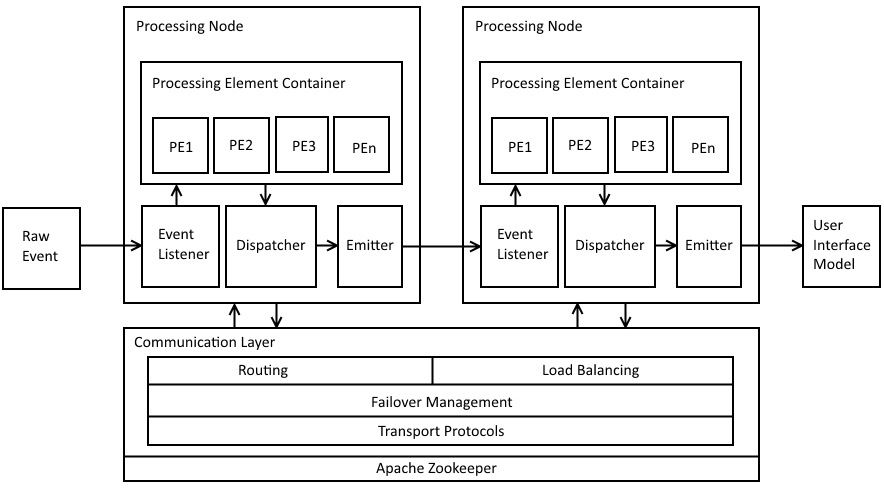
\includegraphics[width=1.0\textwidth]{bilder/s4ProcessingNodes.png}
\caption{Apache S4 Processing Nodes
\label{fig:s4ProcessingNode}}
\end{figure}

In einem \textit{Processing Element} wird die Datenverarbeitung durchgeführt. In Apache S4 gibt es nur zwei Typen von \textit{Processing Elements}, ein Schlüssel-loses und ein Schlüssel-behaftetes \textit{Processing Element}. Der Schlüssel-lose Typ kann unterschiedliche Apache S4 Nachrichten empfangen. Der Schlüssel-behaftete Typ kann nur Apache S4 Nachrichten mit einem definierten Schlüssel in der Nachricht empfangen. Spezielle Aggregate und Operatoren von Nachrichten müssen in \textit{Processing Elements}-Klassen explizit implementiert werden. Ein \textit{Processing Element} besteht aus Zwei Teilen, dem \textit{Prototype} und der \textit{Instance}. Der \textit{Prototype} erbt von der Basisklasse \textit{ProcessingElement} und behandelt eingehende Nachrichten. Die \textit{Instance} erbt von der Basisklasse \textit{App} und behandelt den Anwendungsstart und Anwendungsstop. Im Anhang \ref{lst:s4HelloAppProcessingElementInstance} wird ein Beispiel für das Erzeugen eines \textit{Streams} "`names"' und die Weitergabe der Nachrichten an einen \textit{Stream} gezeigt. \citeint{s4:overview}

\begin{figure}[htb!]
\centering
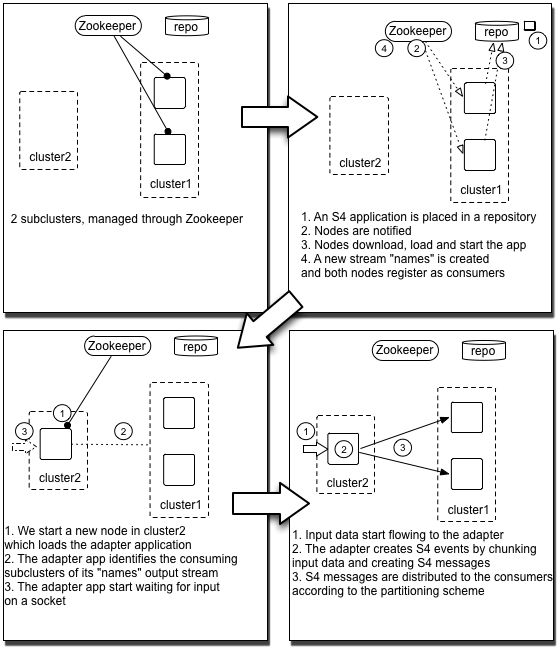
\includegraphics[width=1.0\textwidth]{bilder/s4SampleAppDeployment.png}
\caption{Apache S4 HelloApp Beispiel
\label{fig:s4HelloApp}}
\end{figure}

In Abbildung \ref{fig:s4HelloApp} wird das Beispiel \ref{s4:beispielHelloApp} aus der Apache S4 Installation im Anhang \ref{sec:s4install} gezeigt. Die Abbildung \ref{fig:s4HelloApp} wurde aus der Dokumentation \citeint{s4:walkthrough} entnommen. Zuerst werden Zwei Cluster \textit{cluster1} und \textit{cluster2} in einem Apache Zookeeper \textit{Cluster} bereitgestellt. Anschließend wird im \textit{Repository} die S4 Anwendung \textit{myApp} hinzugefügt. Die Apache S4 \textit{Nodes} werden über Apache Zookeeper informiert und die Anwendung wird gestartet. Ein neuer \textit{Stream} "`names"' wird erstellt und beide \textit{Nodes} werden als \textit{Consumer} registriert. Anschließend wird im \textit{Cluster} \textit{cluster2} die \textit{HelloInputAdapter}-Anwendung gestartet. Beim Bereitstellen der Anwendung im \textit{Cluster} \textit{cluster2} wird der \textit{Stream} "'names"' als Identität für den Ausgabestrom gesetzt. Die \textit{HelloInputAdapter}-Anwendung ist nach dem Starten aktiv und wartet auf Dateneingang. Abschließend werden eintreffende Daten vom \textit{Cluster} \textit{cluster2} in Apache S4-Nachrichten umgewandelt und zur weiteren Datenbehandlung an die \textit{Consumer} verteilt.


Nachrichten werden in Apache S4 zwischen den \textit{Nodes} durch den \textit{Communication Layer} übertragen. Der \textit{Communication Layer} nutzt für die Koordination der Nachrichten zwischen den Apache S4 \textit{Nodes} Apache Zookeeper. Um Nachrichten an die \textit{Nodes} im Apache S4 \textit{Cluster} zu senden, können spezielle Bindungen in verschiedenen Programmiersprachen implementiert werden. Durch ein steckbares Design können unterschiedliche Nachrichtenprotokolle wie zum Beispiel Apache Avro oder Apache Thrift eingesetzt werden. Eine Implementierung für das \gls{glo:udp} \citeint{s4:classUdpEmitter} und dem \gls{glo:tcp} \citeint{s4:classTcpEmitter} wird von Apache S4 bereits unterstützt. \citelit[S. 4, Kap. II D]{s4:Neumeyer}

Die Fehlertoleranz in Apache S4 wird durch die \textit{Fail-Fast} Strategie von Apache Zookeeper übernommen. In einem Apache S4 Cluster mit Zwei \textit{Tasks} und Vier gestarteten \textit{Nodes}, sind Zwei \textit{Nodes} Aktiv und Zwei \textit{Nodes} im \textit{Standby}-Betrieb. Wenn Apache Zookeeper einen \textit{Session-Timeout} einer aktiven \textit{Node} feststellt, wird sofort eine \textit{Standby-Node} aktiviert. Die anderen \textit{Nodes} werden durch den \textit{Communication Layer} über neue aktive \textit{Node} informiert und neue Nachrichten werden umgeleitet. Apache S4 \textit{Nodes} nutzen für die Datenverarbeitung den lokalen Speicher von Apache Zookeeper. Im Fehlerfall geht der Zwischenspeicher einer Apache Zookeeper \textit{Node} verloren. Damit die Daten nicht verloren gehen, kann mit dem \textit{Checkpointing}-Mechanismus über die Konfiguration eine Datensicherung in einem externen Datenlager erfolgen. Beim Start der neuen \textit{Nodes} aus dem \textit{Standby}-Betrieb kann die Datensicherung in den lokalen Speicher zurückgeschrieben werden. In \citelit{valles2012analysis} untersucht Vall{\'e}s verschiedene Ansätze von \textit{Checkpointing} und zeigt eine geringe Performanz der Standardimplementierung gegenüber einer Implementierung mit Apache HBase\footnote{Apache HBase ist eine Apache Hadoop Datenbank, ein verteilter, skalierbarer Big Data-Speicher \citeint{hbase:home}.}. \citeint{s4:faultTolerance}

\begin{table}[!ht]
	\centering
		\begin{tabular}{@{}ll@{}} \toprule
			\textbf{Kriterium} & \textbf{Bewertung} \\ \midrule
			Architektur & Strukturierte Peer-to-Peer-Architektur \\
			Prozesse und Threads & Client-Server-Modell \\
			Kommunikation & TCP-basiert und UDP-basiert via Apache Zookeeper \\
			Namenssystem & Hierarchische Benennung \\
			Synchronisierung & Communication Layer \\
			Pipelining und Materialisierung & Chaining von Processing Elements  \\
			Konsistenz und Replikation & Consistent hashing, Checkpointing \\
			Fehlertoleranz & Failover und Checkpointing \\ 
			Sicherheit & Nur eigene Maßnahmen \\
			& Monitoring mit JMX pro Node \\
			Erweiterung & Modulare Eigenentwicklung \\
			Qualität & Nur eigene Entwicklung für \gls{glo:qos}  \\
			\bottomrule			
		\end{tabular}
	\caption{Bewertung Apache S4}
	\label{tab:bews4}
\end{table}

Bei der Sicherheit sind eigene Maßnahmen notwendig. Nachrichten werden im Klartext oder binär übertragen. Die Verbindung zwischen den einzelnen \textit{Processing Nodes} findet unautorisiert statt. Für die Autorisierung und Verschlüsselung ist eine spezielle Implementierung des \textit{Communication Layer} und der einzelnen \textit{Processing Elements} notwendig. Weiterhin ist eine Verschlüsselung des lokalen Speichers von Apache Zookeeper in einem offenen Netz zu empfehlen. Über \gls{glo:jmx} können Metriken eines Apache S4 Clusters abgefragt werden \citeint{s4:metrics}. \gls{glo:qos} wird in \citelit[S. 3, Kap. II B]{s4:Neumeyer} als anwendungsspezifisch eingestuft. In einer spezifischen Anwendung muss daher eine eigene Implementierung für das \gls{glo:qos} in Apache S4, innerhalb von \textit{Processing Elements} erfolgen.


Diese Kapitel stellt das Streaming Framework Apache S4 vor. Es wurde die Installation von Apache S4 beschrieben und im Anhang \ref{sec:s4install} eine Anleitung abgelegt. Weiterhin erfolgte eine Erklärung der Architektur und der Informationsfluss in einem Apache S4 \textit{Cluster} wurde erläutert. Es wurde die Fehlertoleranz in Zusammenhang von Apache Zookeeper und die Replikation mit \textit{Checkpointing} beschrieben und zuletzt auf eine geringe Sicherheit, Monitoring und Qualität hingewiesen. Nach der Vorstellung der Streaming Frameworks werden im folgenden Kapitel die wesentlichen Kernelemente der einzelnen Streaming Frameworks zusammengefasst.

\section{Zusammenfassung}